\subsection{Approach A——}
The pseudocode for ... is summarised in Algorithm~\ref{alg:}.  

\begin{algorithm}[htb]
\label{alg:}
\caption{Name} % 算法的名字
\hspace*{0.02in} {\bf Input:} \\% 算法的输入, \hspace*{0.02in}用来控制位置,\\ 换行
\hspace*{0.02in} {\bf Output:} % 算法的结果输出
\begin{algorithmic}[1]

\For{every ...} % For 语句,需要和EndFor对应
  \State ...
  \If{...} % If 语句,需要和EndIf对应
    \State ...
  \Else
    \State ...
  \EndIf
  \State ...
  \For{...}
      \State ... 
      \If{...}
          \State ...
      \Else
          \State ...
      \EndIf
  \State ...
  \If{...}
      \State ...
  \Else
      \State ...
  \EndIf
  \EndFor
\EndFor
\State \Return ...
\end{algorithmic}
\end{algorithm}


\subsubsection{HSV}

\begin{figure}[htb]
    \centering
    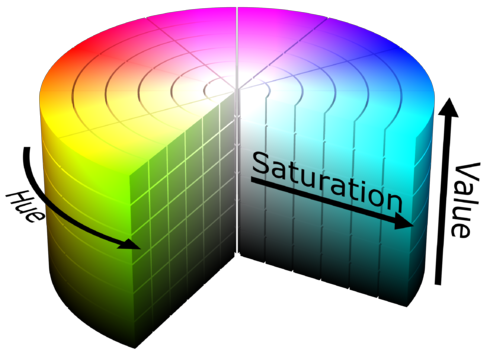
\includegraphics[width=0.35\textwidth]{images/HSV.png}
    \caption{Hue, Saturation, Value colour space (source: \url{https://upload.wikimedia.org/wikipedia})}
    \label{fig:HSV diagram}
\end{figure}

\subsubsection{...}
... The expression is as follows:
\begin{equation}
    d(x, y) = \left\{\begin{matrix}
    &255& \quad if\ lower\ value\le s(x, y)\le higher\ value \\
    &0& \quad otherwise
    \end{matrix}\right.
\end{equation}

where ...

% \subsubsection{Median Filtering}

% \begin{equation}
%     g(x, y) = med\{f(x-k, y-l)\quad  k, l \in W\}
% \end{equation}

% \begin{figure}[htb]
%     \centering
%     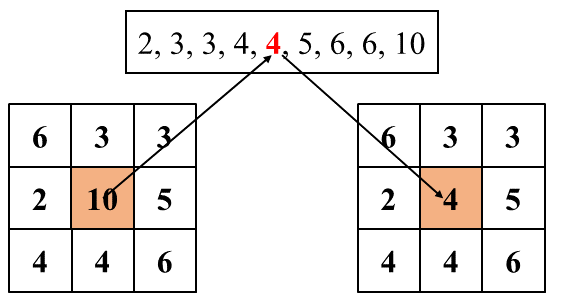
\includegraphics[width=0.4\textwidth]{images/median_filter.png}
%     \caption{Calculation principle of median filtering}
%     \label{fig:princinple of median filtering}
% \end{figure}

\subsubsection{...}
Here you can make some annotations to the equations, see \url{https://github.com/synercys/annotated_latex_equations}

\begin{equation}
    d(x, y) = \eqnmarkbox[blue]{min}{min}_{(x', y')|pixel(x', y')\ne 0}\ s(x+x', y+y')
\end{equation}

\begin{equation}
    d(x, y) = \eqnmarkbox[red]{max}{max}_{(x', y')|pixel(x', y')\ne 0}\ s(x+x', y+y')
\end{equation}

Sub figures.

\begin{figure}[!ht]
    \centering
    \subfigure[Original 'i']{
\includegraphics[width=0.15\textwidth]{images/origin_i.png}}
    \subfigure[Eroded 'i']{
\includegraphics[width=0.15\textwidth]{images/eroded_i.png}}
    \subfigure[Dilated 'i']{
\includegraphics[width=0.15\textwidth]{images/dilated_i.png}}
    \caption{Caption}
    \label{fig:'i'}
\end{figure}




\subsection{Approach B——}
The network structure...

A PowerPoint drawing template for machine learning models, see \url{https://github.com/dair-ai/ml-visuals}

\begin{figure}[!ht]
    \centering
    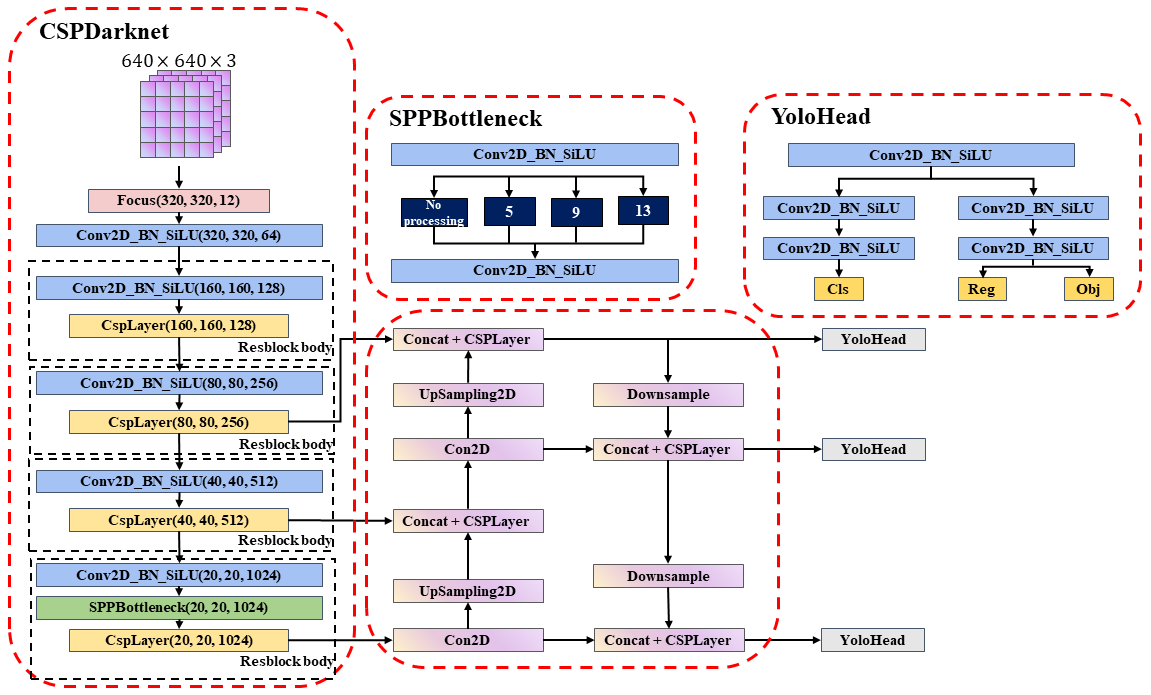
\includegraphics[width=1.1\textwidth]{images/Yolox_structure.png}
    \caption{Caption}
    \label{fig:}
\end{figure}


\subsubsection{CSPDarknet}

\begin{enumerate}
    \item \textbf{...} 
    
    \item \textbf{...} 
    
    \item \textbf{...} 
    
    \item \textbf{...} 
\end{enumerate}


\subsubsection{...}
When the input is $640\times 640\times 3$, ...

